% BASED ON SIGPROC-SP.TEX - VERSION 3.1

\documentclass{acm_proc_article-sp}
\usepackage{graphicx}

\begin{document}

\title{Database Refactorings: Detection and Documentation}

\maketitle

\begin{abstract}
With thes onset of rapid prototyping, agile programming, and many other factors,
modern database schemas are increasingly dynamic.  Database refactorings --
that is, evolutions of a database schema -- are increasingly being studied and
utilized by developers who want/need to improve an existing schema design
without breaking its supported functionality.

\textit{[TODO: more-complete description of refactoring, and differentiation
from an actual schema addition/deletion]}

In this paper, we address the issue of documentation becoming out-of-synch
after a database refactoring.  We develop and examine ways of detecting
database refactorings from two snapshots of a database schema, and incorporate
them into ModelDoc, a wiki-based system we have created that updates itself
when it auto-detects schema changes.  Finally, we explore ways of handling
ambiguities when the intent behind a refactoring is unclear, such as inviting
user-input.
\end{abstract}

\category{H.2.1}{Database Management}{Logical Design} \\
\category{H.4}{Information Systems Applications}{Miscellaneous}
\category{D.2.7}{Software Engineering}{Distribution, Maintenance, and
Enhancement}

\terms{wikis, databased, refactoring, database refactoring, database schema
evolution, documentation, auto-generated documentation}

\section{Introduction}

\ldots

\section{Goals / Contributions}

\ldots

\section{Related Work}

\ldots

\section{ModelDoc}

ModelDoc extends MediaWiki's existing functionality through MediaWiki's
standard extension framework.  ModelDoc currently works with Postgres
databases, but features an extension API for interfacing with other
entity-relational data sources, and potentially non-relational database data
sources as well.

\subsection{Overview}

\textit{[TODO: Shorten overview; restrict primarily to refactoring-facing
pieces]}

ModelDoc is MediaWiki extension, built using PHP5 and deployed into an existing
MediaWiki installation using the standard procedure.  Unlike wikis that
encourage more open collaboration, though, a ModelDoc-enabled wiki for a
proprietary project will likely involve stronger security considerations.

Database metadata is obtained via live database connections.  A single ModelDoc
installation can work with an arbitrary number of databases -- the
configuration for these connections is stored in a special ModelDoc wiki page
(see Special Pages).

Members of a project use the wiki in the standard way, collaborating through
the creation and updating of wiki pages.  All the standard wiki-functionality
is maintained and encouraged: version-history for pages, using the
``discussion'' pages for meta-documentation of a page, ``watching'' pages to be
notified when they are updated, etc.

ModelDoc extends MediaWiki, however, with special tags that users can use when
creating documentation.  For example, by adding an ``entity-list'' tag to a
page, and specifying a data source (see Tags section), when later viewing that
page, ModelDoc will query the data source and generate a list of the tables in
that database.  Further, each entry in this list will be a link to a
ModelDoc-generated page containing the table's metadata (columns,
constraints, etc.) and documentation.

For each of these entity-pages, ModelDoc also creates a corresponding HISTORY
page containing -- in XML format -- the last-seen set of metadata for the
table.  This metadata is compared to the live data every time the tag generates
content; ModelDoc compares this information to see what has been added and what
is missing, and appends these changes to the respective pages.  Thus, when
viewing an entity-page, the user sees not only the current information for the
database table, but also an auto-generated history of how that table has
evolved over time.  These sections are editable, the project members can (and
are encouraged to -- see the Special Pages section for ``ModelDoc::To Document''
) update/replace these sections with documentation that is more comprehensive
and user-friendly.

\begin{figure}[b]
\centering
%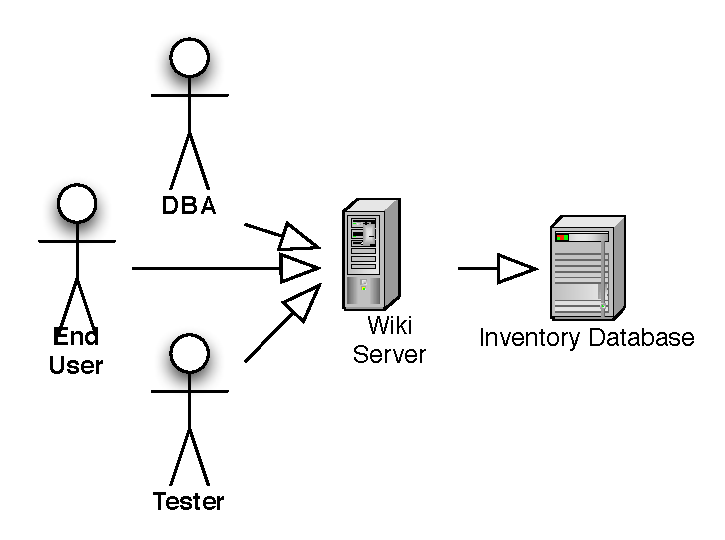
\epsfig{file=Overview.pdf}
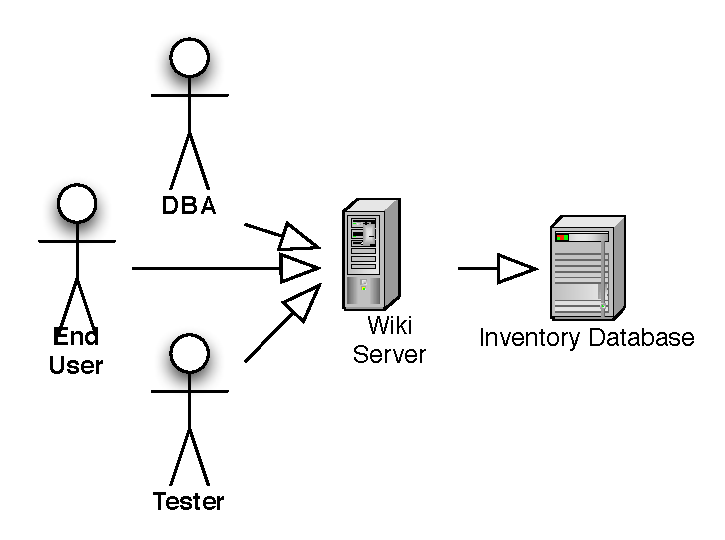
\includegraphics[width=220px]{Overview.pdf}
\caption{Overview of a sample ModelDoc system.}
\end{figure}

\begin{figure}
\centering
%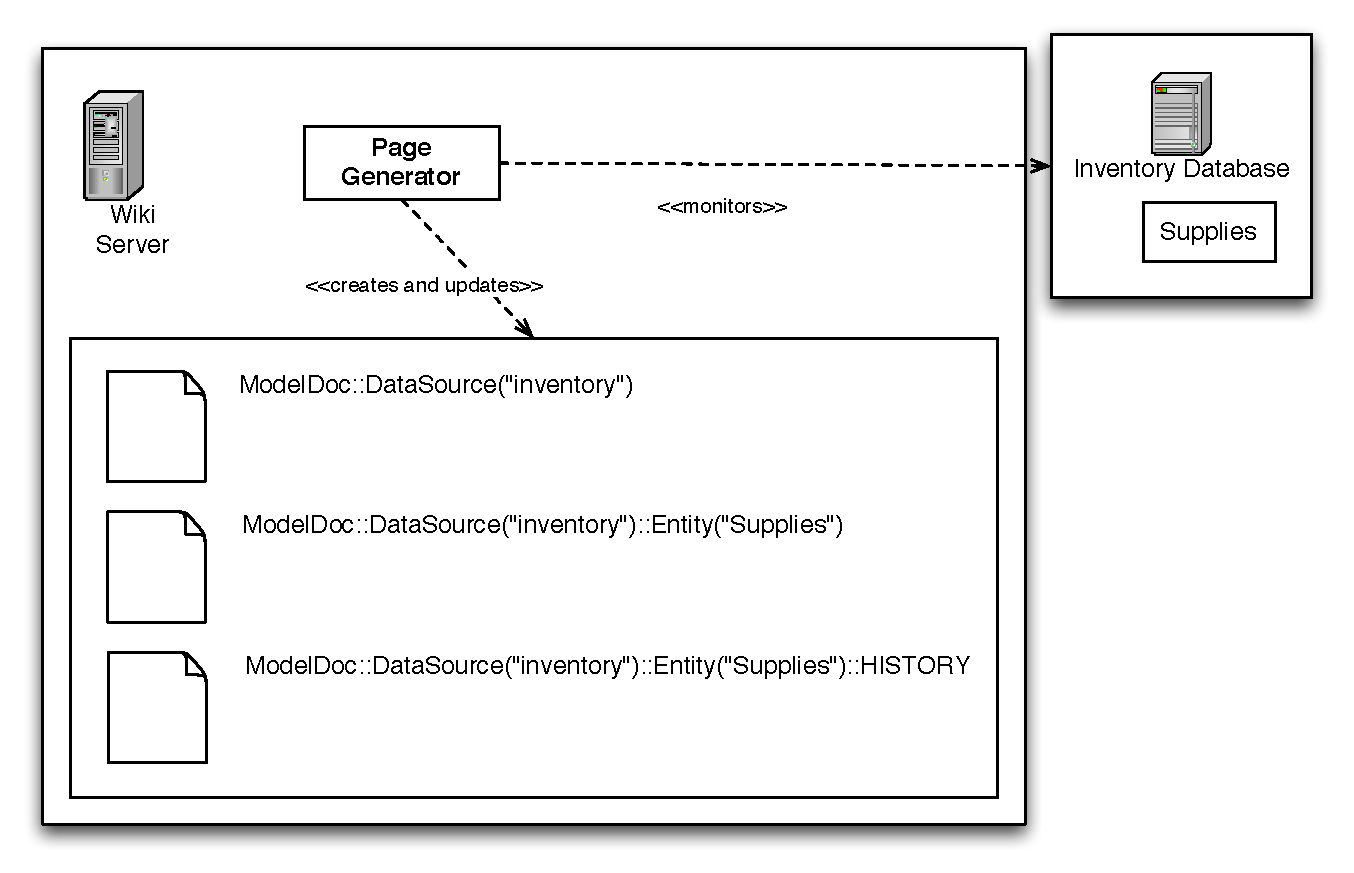
\epsfig{file=PageManager.pdf}
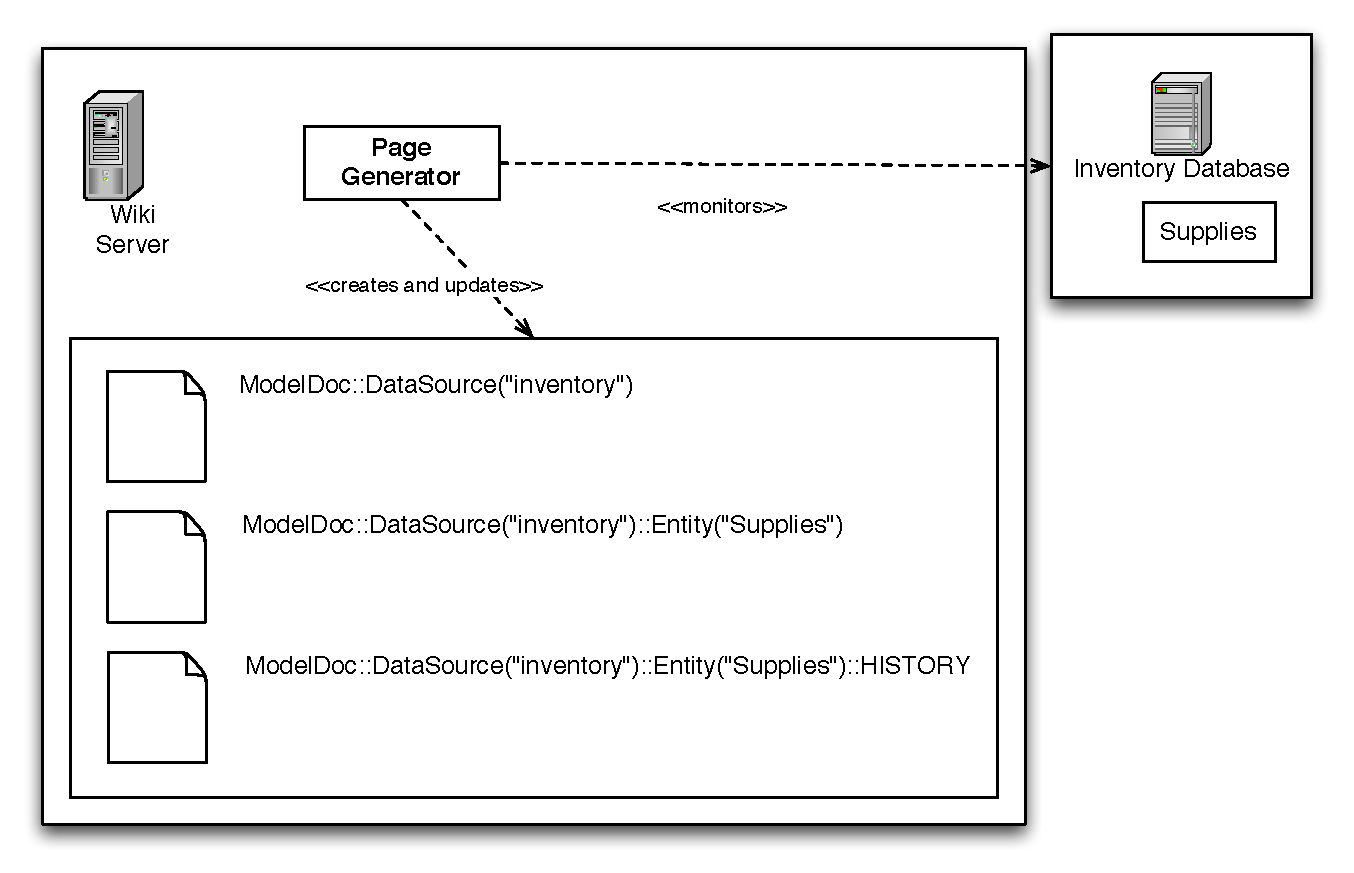
\includegraphics[width=220px]{PageManager.pdf}
\caption{The role of ModelDoc's page-manager component.}
\end{figure}

\subsection{Refactoring Detection}

\ldots

\subsubsection{Detection Process}

\ldots

\subsubsection{Handling Ambiguity}

\ldots

\subsection{Usage}

\ldots

\section{Evaluation}

We used refactorings from \cite{ambler:refactoring} to both illustrate where
ModelDoc currently stands and where it can go with regard to where it can be
used in a database's evolution.

[TODO: Challenges: capture refactorings that deal with data itself, such as new
semantics or data-formats;  detect refactorings that
are made up of both column and table changes, such as the ``Replace Type Code
With Property Flags'' refactoring, which entails replacing a single
``code''-type column with multiple boolean columns, e.g. replacing an
``AddressType'' column with ``isHomeAddress'', ``isWorkAddress'', etc. columns;
  stored procedures ]

\subsection{Structural Refactorings}

ModelDoc documents structural changes well.

\subsubsection{Drop Column}

\ldots

\subsubsection{Drop Table}

\ldots

\subsubsection{Drop View}

\ldots

\subsubsection{Introduce Calculated Column}

\ldots

\subsubsection{Introduce Surrogate Key}

\ldots

\subsubsection{Merge Columns}

\ldots

\subsubsection{Merge Tables}

\ldots

\subsubsection{Move Column}

\ldots

\subsubsection{Rename Column}

\ldots

\subsubsection{Rename Table}

\ldots

\subsubsection{Rename View}

\ldots

\subsubsection{Replace LOB With Table}

\ldots

\subsubsection{Replace Column}

\ldots

\subsubsection{Replace 1-to-Many With Assoc. Tbl}

\ldots

\subsubsection{Replace Surrogate Key With Natural Key}

\ldots

\subsubsection{Split Column}

\ldots

\subsubsection{Split Table}

\ldots

\subsection{Data Quality Refactorings}

\textit{[TODO: Overview and general conclusions]}

\subsubsection{Add Lookup Table}

\ldots

\subsubsection{Apply Standard Codes}

\ldots

\subsubsection{Apply Standard Type}

\ldots

\subsubsection{Consolidate Key Strategy}

\ldots

\subsubsection{Drop Column Constraint}

\ldots

\subsubsection{Drop Default Value}

\ldots

\subsubsection{Drop Non-Nullable Constraint}

\ldots

\subsubsection{Introduce Column Constraint}

\ldots

\subsubsection{Introduce Common Format}

\ldots

\subsubsection{Introduce Default Value}

\ldots

\subsubsection{Make Column Non-Nullable}

\ldots

\subsubsection{Move Data}

\ldots

\subsubsection{Replace Type Code With Property Flags}

\ldots

\subsection{Referential Integrity Refactorings}

\textit{[TODO: Overview and general conclusions]}

\subsubsection{Add Foreign Key Constraint}

\ldots

\subsubsection{Add Trigger For Calculated Column}

\ldots

\subsubsection{Drop Foreign Key Constraint}

\ldots

\subsubsection{Introduce Cascading Delete}

\ldots

\subsubsection{Introduce Hard Delete}

\ldots

\subsubsection{Introduce Soft Delete}

\ldots

\subsubsection{Introduce Trigger For History}

\ldots


\subsection{Architectural Refactorings}

\textit{[TODO: Overview and general conclusions]}

\subsubsection{Add CRUD Methods}

\ldots

\subsubsection{Add Mirror Table}

\ldots

\subsubsection{Add Read Method}

\ldots

\subsubsection{Encapsulate Table With View}

\ldots

\subsubsection{Introduce Calculation Method}

\ldots

\subsubsection{Introduce Index}

\ldots

\subsubsection{Introduce Read-Only Table}

\ldots

\subsubsection{Migrate Method From Database}

\ldots

\subsubsection{Migrate Method To Database}

\ldots

\subsubsection{Replace Method(s) With View}

\ldots

\subsubsection{Replace View With Method(s)}

\ldots

\subsubsection{Use Official Data Source}

\ldots


\subsection{Transformations}

\textit{[TODO: Overview and general conclusions]}

\subsubsection{Insert Data}

\ldots

\subsubsection{Introduce New Column}

\ldots

\subsubsection{Introduce New Table}

\ldots

\subsubsection{Introduce View}

\ldots

\subsubsection{Update Data}

\ldots

\section{Future Work}

\subsection{Free-Text Documentation Refactorings}

To achieve mutual-consistency between the human documentation and the database
metadata, ModelDoc could be extended to infer, for example, that a user is
referring to a given entity even on a non-ModelDoc page.  If that entity
is refactored/transformed, ModelDoc could then notify the user that this other
documentation may also need to be updated.

[TODO: Flesh out]

\subsection{Suggesting Client Code Refactorings}

The model of an application is rarely exclusively contained in the database
schema.  Most applications contain an object model that abstracts on top of the
data model.  For example, as previously discussed, in a database a Person
entity and its associated Address may be normalized into two tables.  In an
accompanying object-oriented application, however, this relationship would take
the form of a Person object composed with an Address object.

When refactorings/transformations are detected, it would be desirable for the
impact of those changes on the client code to also be detected, and for a
system to then suggest changes to client SQL code and ORM configuration.

\subsection{Ability to Mutate Data Sources}

There is little current tool-support for performing database refactoring
\cite{ambler:refactoring}.  Instead of documenting in a read-only way, ModelDoc
could be used to allow mutation of the underlying data sources, including
carrying out complex refactorings.  This would allow ModelDoc to know for sure
that such refactorings were intended -- a column-rename, for example, would no
longer be seen as a column-deletion and column-addition.

\section{Conclusions}

\ldots

\bibliographystyle{abbrv}
\bibliography{modeldoc}
\balancecolumns

\end{document}
